% Fixed coordinate tests eventually read zero on the unit vectors.
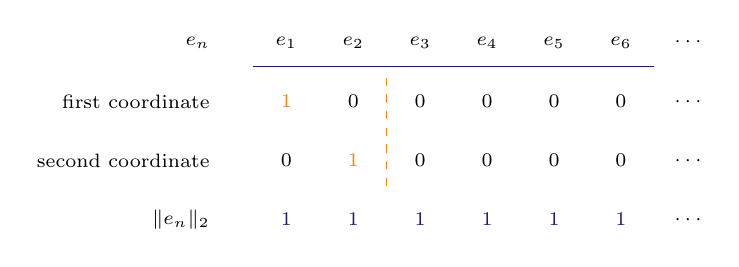
\begin{tikzpicture}[x=0.85cm,y=0.75cm,every node/.style={font=\scriptsize}]
\node[anchor=east] at (0,0) {$e_n$};
\node[anchor=east] at (0,-1) {first coordinate};
\node[anchor=east] at (0,-2) {second coordinate};
\node[anchor=east] at (0,-3) {$\|e_n\|_2$};
\foreach \n in {1,...,6}{
\node at (\n,0) {$e_{\n}$};
\node[MidnightBlue] at (\n,-3) {$1$};
}
\foreach \n in {2,...,6}{\node at (\n,-1) {$0$};}
\foreach \n in {1,3,4,5,6}{\node at (\n,-2) {$0$};}
\node[BurntOrange] at (1,-1) {$1$};
\node[BurntOrange] at (2,-2) {$1$};
\draw[MidnightBlue] (0.5,-0.4)--(6.5,-0.4);
\draw[BurntOrange,dashed] (2.5,-0.6)--(2.5,-2.5);
\node at (7,0) {$\cdots$};
\node at (7,-1) {$\cdots$};
\node at (7,-2) {$\cdots$};
\node at (7,-3) {$\cdots$};
\end{tikzpicture}
